\documentclass[../main.tex]{subfiles}

\usepackage{nopageno} %Seitenzahlen auf richtiger Seite 

\usepackage[left=2cm, right=2cm, top=2cm, includehead, includefoot, headheight=17pt]{geometry}

\usepackage[utf8x]{inputenc}
\usepackage[english]{babel}
\usepackage{amsmath,amssymb,amsthm}
\usepackage{framed}
\usepackage{wasysym}
\usepackage[T1]{fontenc} %Silbentrennung 
\usepackage{color} %Farbe
\usepackage{graphicx}
\usepackage{float}%Grafik am gleichen Ort plazieren
%pdf. png. einfach eingliedern
\usepackage{subfigure} %Grafiken nebeneinander
\usepackage{pdfpages}
\usepackage{ulem} 	%\uuline{urgent}    % doppelt unterstreichen
%\uwave{boat}      % unterschlängeln
%\sout{wrong}       % durchstreichen
%\xout{removed}     % ausstreichen mit //////.

\usepackage{tikz}
\usetikzlibrary{trees}
\usetikzlibrary{plotmarks}
\usetikzlibrary{angles,quotes,babel}
\usetikzlibrary{shadings}
\usetikzlibrary{patterns}
\usetikzlibrary{matrix}
\usetikzlibrary{arrows}
\usetikzlibrary{calc}

\usepackage{pgfplots}
\usepackage{pgf-pie}
\pgfplotsset{compat=1.10}
\usepgfplotslibrary{statistics}
\usepgfplotslibrary{fillbetween}

\usepackage{tkz-euclide}
\usepackage{enumerate}
\usepackage{stmaryrd}
\usepackage{tabularx}
\usepackage{wrapfig}
\usepackage{epsdice}
\usepackage{multirow}
\usepackage{rotating}
\usepackage{pdflscape}
\usepackage{fancyhdr}

\pagestyle{fancy} %eigener Seitenstil
\fancyhf{} %alle Kopf- und Fußzeilenfelder bereinigen
\fancyhead[L]{} %Kopfzeile links
\fancyhead[C]{} %zentrierte Kopfzeile
\fancyhead[R]{} %Kopfzeile rechts
\renewcommand{\headrulewidth}{0.4pt} %obere Trennlinie
\fancyfoot[C]{\thepage} %Seitennummer
\renewcommand{\footrulewidth}{0.4pt} %untere Trennlinie

% Number spaces 
\newcommand{\CC}{\ensuremath{\mathbb{C}}}
\newcommand{\RR}{\ensuremath{\mathbb{R}}}
\newcommand{\QQ}{\ensuremath{\mathbb{Q}}}
\newcommand{\ZZ}{\ensuremath{\mathbb{Z}}}
\newcommand{\NN}{\ensuremath{\mathbb{N}}}
\newcommand{\LL}{\ensuremath{\mathbb{L}}}
\newcommand{\DD}{\ensuremath{\mathbb{D}}}
\newcommand{\WW}{\ensuremath{\mathbb{W}}}

%draw chemestry molecules 
\usepackage{chemfig} % https://mirror.ox.ac.uk/sites/ctan.org/macros/generic/chemfig/

\newcommand\vv[1]{%
	\begin{tikzpicture}[baseline=(arg.base)]
		\node[inner xsep=0pt] (arg) {$#1$};
		\draw[line cap=round,line width=0.45,->,shorten >= 0.2pt, shorten <= 0.7pt] (arg.north west) -- (arg.north east);
	\end{tikzpicture}%
} %command will render \vv{x} with an arrow aboth 

\renewcommand{\labelenumi}{\roman{enumi})}

\DeclareMathOperator{\ggT}{ggT}
\DeclareMathOperator{\sign}{sign}

%sections
\theoremstyle{plain}
\newtheorem{Thm}{Theorem}[section]
\newtheorem{Def}[Thm]{Definition}
\newtheorem{Prop}[Thm]{Proposition}

\theoremstyle{definition}
\newtheorem{lemma}[Thm]{Lemma}
\newtheorem{corollary}[Thm]{Corollary}
\newtheorem{claim}[Thm]{Claim}
\newtheorem{Proof}[Thm]{Proof}
\newtheorem{Ex}[Thm]{Example}

\newtheorem{Exercise}{ex}[section] %follow proper enum
\newtheorem{ex}[Exercise]{Exercise}
\newtheorem{Solution}{sol}[section]
\newtheorem{sol}[Solution]{Solution}

\theoremstyle{remark}
\newtheorem{remark}[Thm]{Remark} % follows thm enum

\newtheorem{comment}{Comment}[section] %follow comment enum
\newtheorem{notation}[comment]{Notation}
\newtheorem{reasoning}[comment]{Reasoning}
\newtheorem{Intpr}[comment]{Interpretation}

%some premmade with title (uterwise use \textbf{Title} ...)
\newenvironment{ThmWithTitle}[1]{%
	\begin{Thm}[\textbf{#1}]}{\end{Thm}}
\newenvironment{PropWithTitle}[1]{%
	\begin{Prop}[\textbf{#1}]}{\end{Prop}}
\newenvironment{ExWithTitle}[1]{%
	\begin{Ex}[\textbf{#1}]}{\end{Ex}}
\newenvironment{DefWithTitle}[1]{%
	\begin{Def}[\textbf{#1}]}{\end{Def}}
\newenvironment{RemarkWithTitel}[1]{%
	\begin{remark}[\textbf{#1}]}{\end{remark}}

%format of paragraph 
\renewcommand\paragraph{\@startsection{paragraph}{4}{\z@}%
	{-2.5ex\@plus -1ex \@minus -.25ex}%
	{1.25ex \@plus .25ex}%
	{\normalfont\normalsize\bfseries}}
\makeatother
\setcounter{secnumdepth}{4} % how many sectioning levels to assign numbers to
\setcounter{tocdepth}{4}    % how many sectioning levels to show in ToC

\newcounter{row} 
\renewcommand\therow{\alph{row}} %hier a,b,c etc. def und mit therow abrufbar

\newenvironment{aufz}
{\setcounter{row}{0}%
	\par\noindent\tabularx{\linewidth}[t]
	{\cdot{20}{>{\stepcounter{row}\makebox[1.5em][l]{\therow)\hfill}}X}} %bis max 20 Elemente nebeinander
}
{\endtabularx}


%biblio
\usepackage[]{biblatex}
\addbibresource{referenzenma.bib} 

%glossary
\usepackage{glossaries}
\usepackage{import}


\usepackage{rotating} % Include this package in the preamble

\newglossaryentry{FRAP}{
    name={FRAP},
    description={\textbf{Fluorescence Recovery After Photobleaching}. A microscopy technique used to study the dynamics of molecular diffusion and protein mobility within cells. The method involves selectively bleaching a fluorescently labeled region using a high-intensity laser and monitoring fluorescence recovery over time as unbleached molecules move into the area. The recovery rate provides insights into molecular diffusion, binding interactions, and membrane fluidity.}
}


\newglossaryentry{phosphoglycerols}{
    name={Phosphoglycerols},
    description={A class of phospholipids derived from glycerol-3-phosphate. They form a major component of biological membranes and typically consist of a glycerol backbone, two fatty acid chains, and a phosphate group attached to a polar head. Examples include phosphatidylcholine and phosphatidylserine.}
}

\newglossaryentry{sphingolipids}{
    name={Sphingolipids},
    description={A class of lipids that contain a sphingosine backbone instead of glycerol. They play crucial roles in cell membrane structure and signaling. Key sphingolipids include ceramides, sphingomyelins, and glycosphingolipids, which are involved in cellular communication and recognition processes.}
}

\newglossaryentry{phosphatidylinositol}{
    name={Phosphatidylinositol (PI)},
    description={A phospholipid that plays a key role in cell signaling and membrane dynamics. It consists of a glycerol backbone linked to two fatty acid chains and a phosphate group attached to an inositol ring. Phosphatidylinositol and its phosphorylated derivatives (phosphoinositides) are involved in intracellular signaling pathways, membrane trafficking, and cytoskeletal organization.}
}


\newglossaryentry{lateralphaseseparation}{
    name={Lateral Phase Separation},
    description={A phenomenon in biological membranes where different lipid and protein components segregate into distinct coexisting phases within the same membrane plane. This separation can lead to the formation of specialized microdomains, such as lipid rafts, which influence membrane fluidity, signaling, and protein localization. Lateral phase separation is driven by differences in lipid composition, temperature, and molecular interactions.}
}



\makeglossaries

\begin{document}
    \section{Membrane Structure}

        \subsection{Introduction to Cell Membranes}
            
        \begin{figure}[H]
            \centering
             % First subfigure (side by side)
            \subfigure[membrane structure]{
                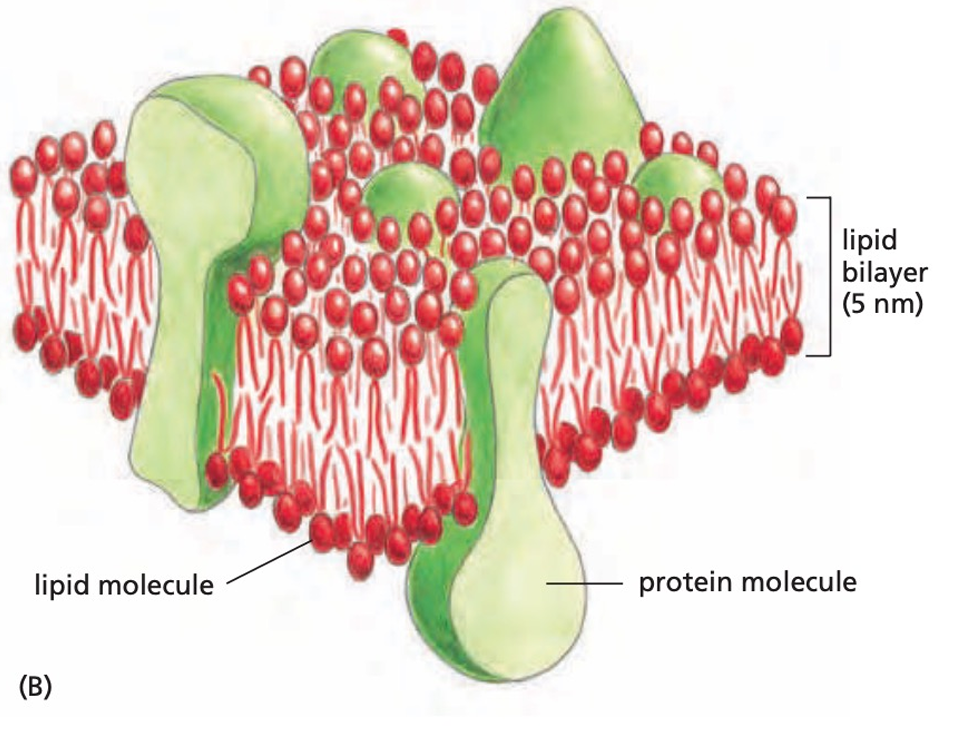
\includegraphics[width=0.45\linewidth]{lipid_membrane_structure.png}
                \label{fig:MembrStruct}
            }
            \hspace{0.05\textwidth} % Adds a small horizontal space between the figures
            % Second subfigure (side by side)
            \subfigure[sigmoid binding curve]{
                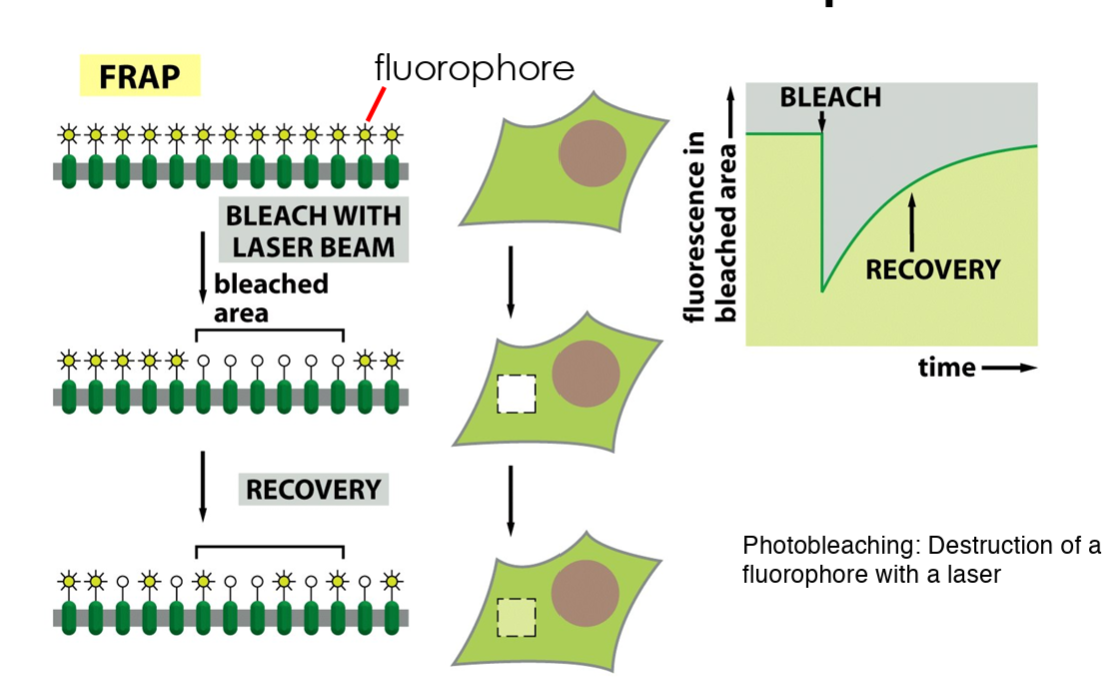
\includegraphics[width=0.45\linewidth]{FRAP.png}
                \label{fig:FRAP}
            }
            \caption{Membrane structure and fluid property}
            \label{fig:ITC_all}
        \end{figure}

        Cell membranes consist of a \textbf{lipid bi-layer} and various membrane proteins. This relatively simple structure has very important functions such as \textbf{protecting the cytosol} and the chemistry of the cell from the outside. This is very improtant as it allows the cell to have a different chemical enviroment than the outside. The cell is also  \textbf{membrane is a liquid }which can be seen by \textbf{\gls{FRAP}} experiments. THe frap experiment works as follows:
        \begin{enumerate}
            \item tag membrane with GFP
            \item shoot powerful laser that bleaches the flouresent protein (stops being green)
            \item observe how the affected area recovers. How fast the area statrs glowing again gives info on the diffusion constant and by extent the mobility of the tagged molecules.
        \end{enumerate}

        This \textbf{liquid property can be used by the cell to deform the membrane at will.}

        \subsection{lipid Composition of Cell Membranes}
        \begin{figure}[H]
            \centering
            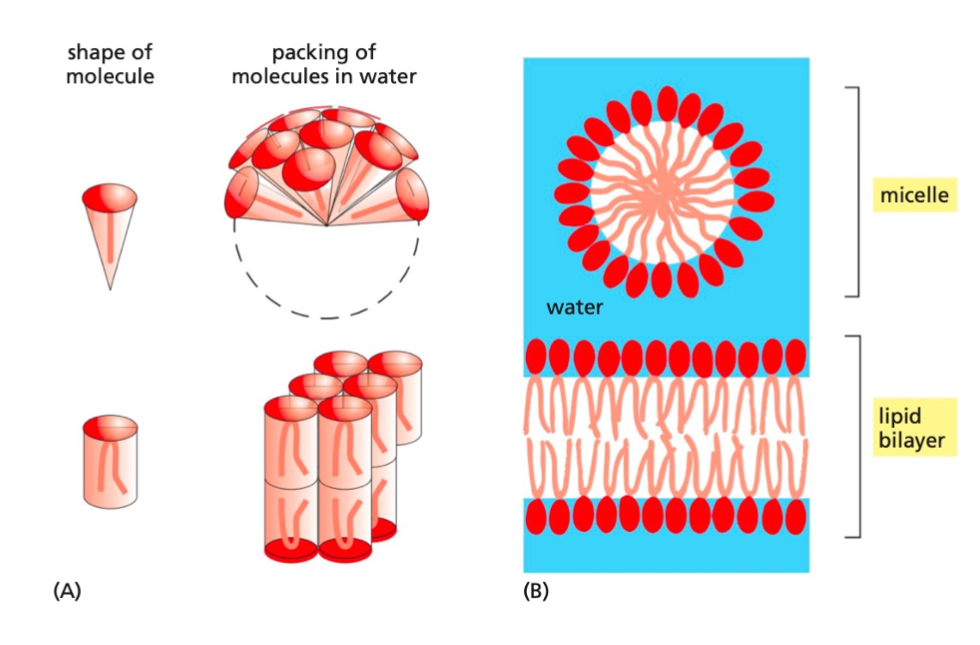
\includegraphics[width=0.5\linewidth]{biLayer.png}
            \caption{spontaneous formation of lipid bi layer}
            \label{fig:bilayer}
        \end{figure}
        Phospholipids make up majority of lipids in the membrane Phospholipids are \textbf{amphiphilic}. They have a hydrophilic head and hydrophobic tail. The lipid structure that forms depends to a very large extent on the 3D structrue of the lipid. If the lipid only has 1 hydrophobic tail it will form globules called \textbf{miscelles} however if it has 2 it will form a \textbf{bi-layer}. This lipid bi-layer has the unique property that it \textbf{will self seal into a closed membrane} as this is the most energetically favorable state. 

        \begin{remark}
            The property of the molecule two seal off means that if pierced it will reform giving it the \textbf{ability of self repair}
        \end{remark}

        \subsubsection{types of lipids in membrane}
        The lipids in a cell membrane are very diverse but can be divided into 3 classes: phospholipids, glycolipds and sterols.
            \begin{figure}[H]
                \centering
                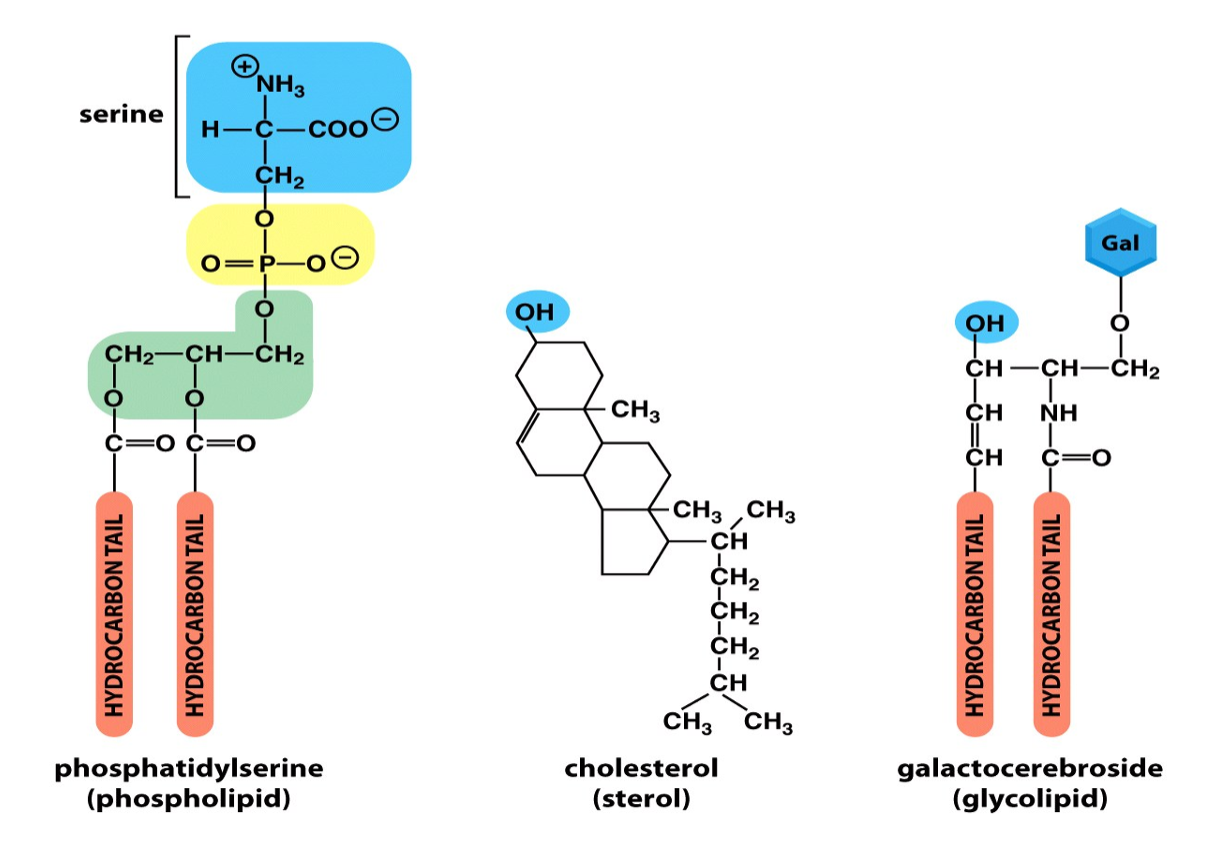
\includegraphics[width=0.6\linewidth]{typesLipids.png}
                \caption{3 main classes of lipids}
                \label{fig:lipids}
            \end{figure}
            
        \paragraph{phospholipids}

            \begin{figure}[H]
                \centering
                 % First subfigure (side by side)
                \subfigure[4 main phospholipids]{
                    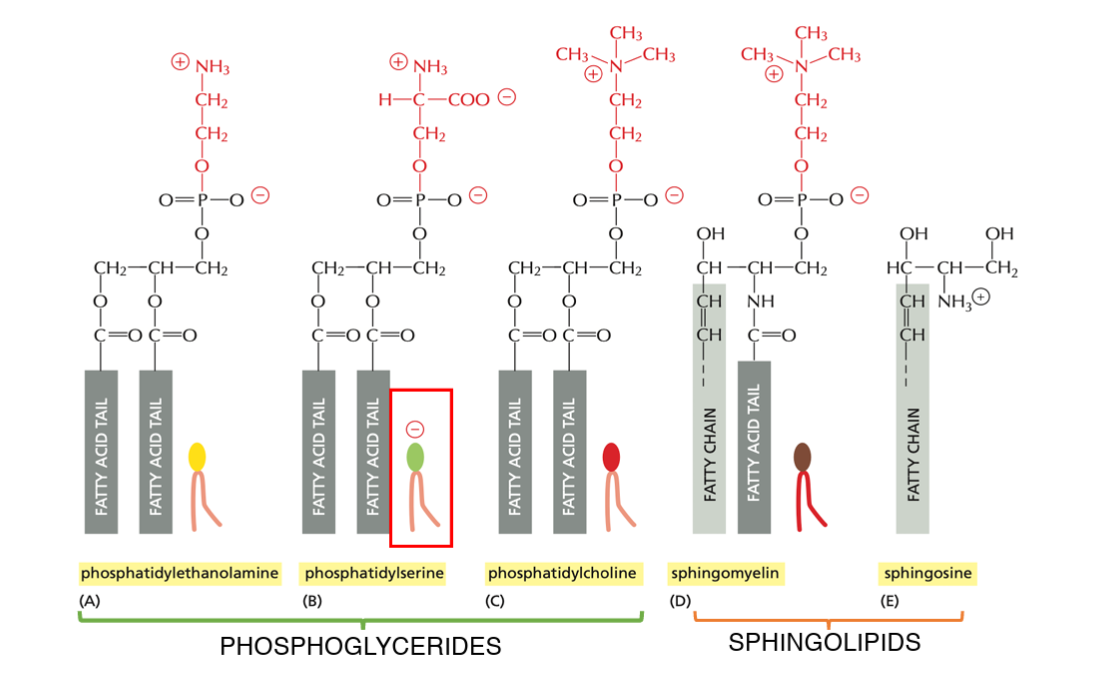
\includegraphics[width=0.55\linewidth]{phospholipids.png}
                    \label{fig:phospholipids}
                }
                \hspace{0.05\textwidth} % Adds a small horizontal space between the figures
                % Second subfigure (side by side)
                \subfigure[phospholipids vs sphingolipids]{
                    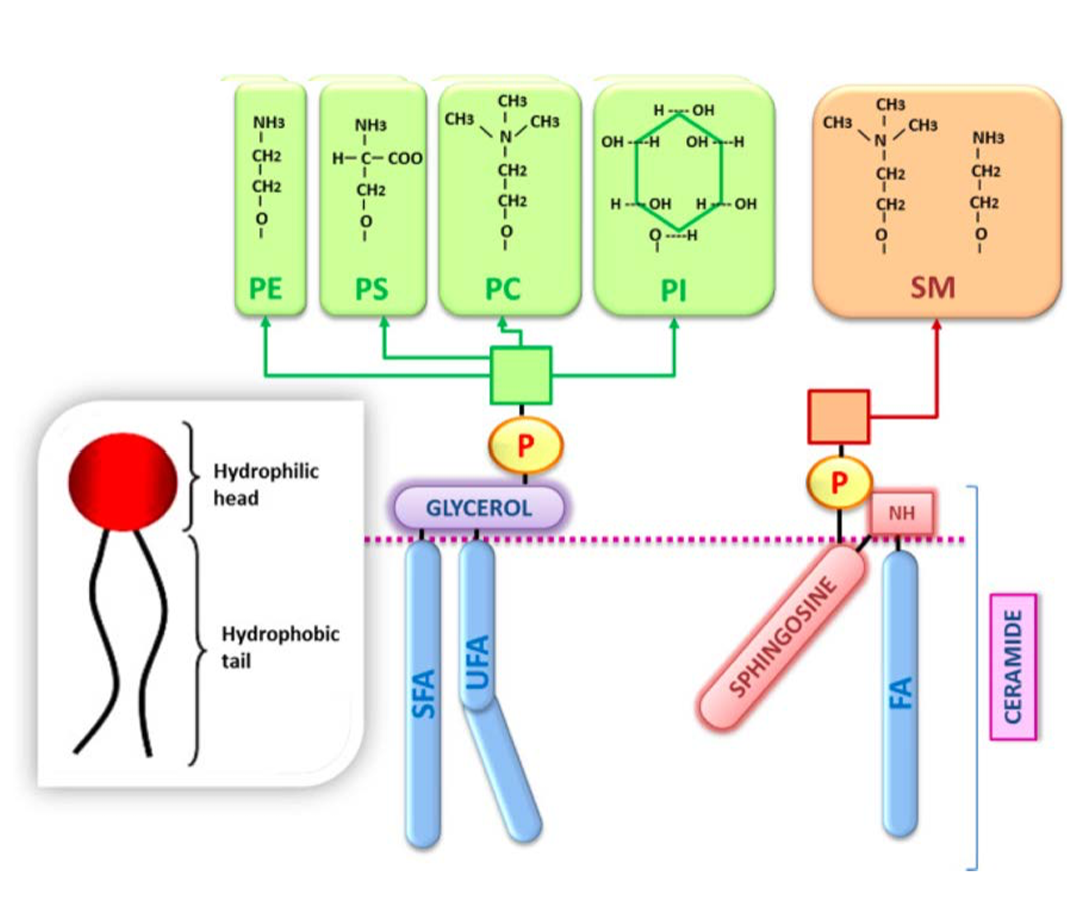
\includegraphics[width=0.35\linewidth]{sphingosine.png}
                    \label{fig:PhospholipisVsSphingolipids}
                }
                \caption{PI can be phosphorilated based on location}
                \label{fig:ITC_all}
            \end{figure}
         
            the main lipids in a membrane are phospholipids. These consist of a glycerol backbone and a phosphate attached.
            There are four main phospholipids in our cells are:
            \begin{enumerate}
                \item phosphatidylethanolamine (PE)
                \item phosphatidylserine (PS)
                \item phosphatidylcholine (PC)
                \item sphigomyelin
                \item sphigosine
            \end{enumerate}

        These can be further divided into \textbf{\gls{phosphoglycerols}} and \textbf{\gls{sphingolipids}}. Each of these have a different backbone where phosphoglycerols have a \textbf{ glycerol} backbone and sphinolipids have a \textbf{sphingosine} backbone plus a \textbf{ceramide}. Sphingolipids can be modified in two different ways, they can be modified into \textbf{glycosphingolipids} or \textbf{phosphosphingolipids}.

        \subparagraph{Phosphatidylinosito (PI)}
        \begin{figure}[H]
            \centering
             % First subfigure (side by side)
            \subfigure[the 8 PI phosphorilations]{
                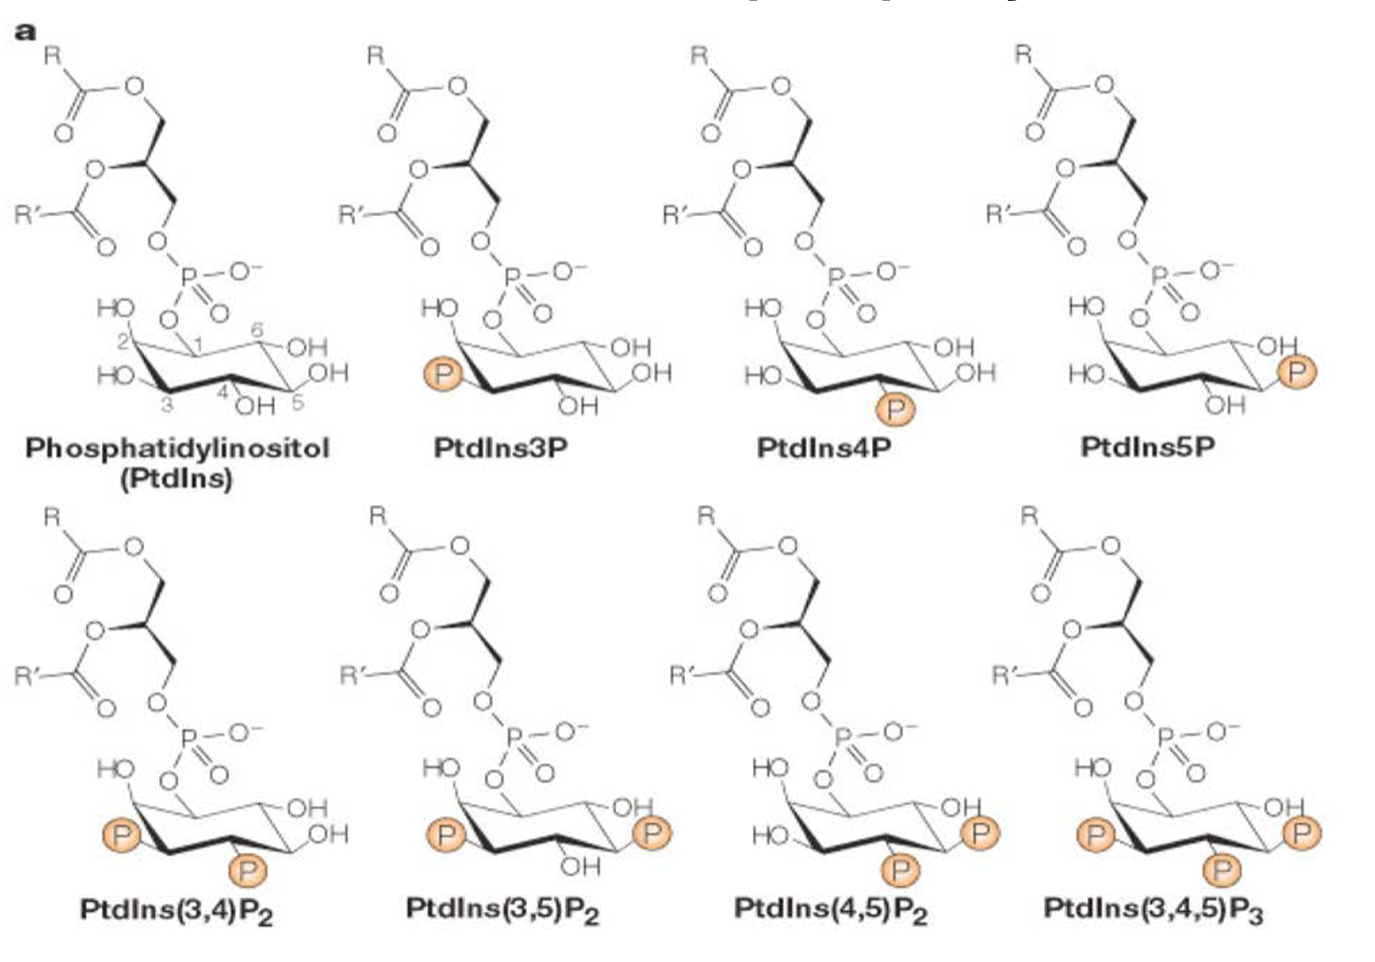
\includegraphics[width=0.45\linewidth]{PI_overview.png}
                \label{fig:MembrStruct}
            }
            \hspace{0.05\textwidth} % Adds a small horizontal space between the figures
            % Second subfigure (side by side)
            \subfigure[PI locations]{
                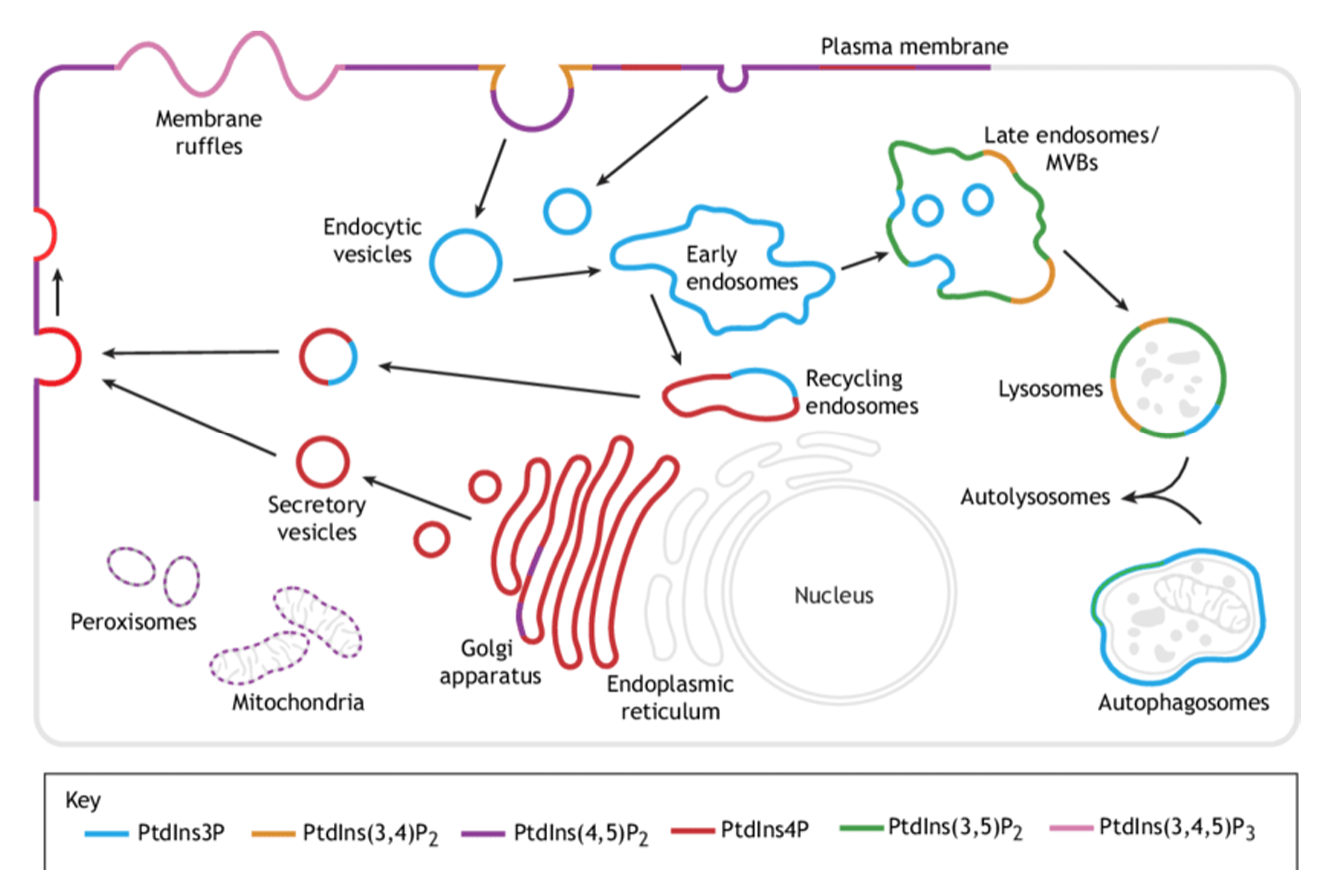
\includegraphics[width=0.45\linewidth]{pI_location.png}
                \label{fig:FRAP}
            }
            \caption{PI can be phosphorilated based on location}
            \label{fig:ITC_all}
        \end{figure}
        
        \gls{phosphatidylinositol} is a special phospholipid that is involved in cell signaling it is not one of the main phospholipids but is still important. \textbf{These lipids are located on the iintracellular leaflet (facing inside the cell) }  This can then be used for localization by interaction with various proteins that bind to or phosphorylate PI. (see chapter on cellular localization)
        \begin{remark}
          \textbf{  PI are not a sugar but an alcohol}
        \end{remark}
        
        
        \paragraph{glycolipids}
        \begin{figure}[H]
            \centering
            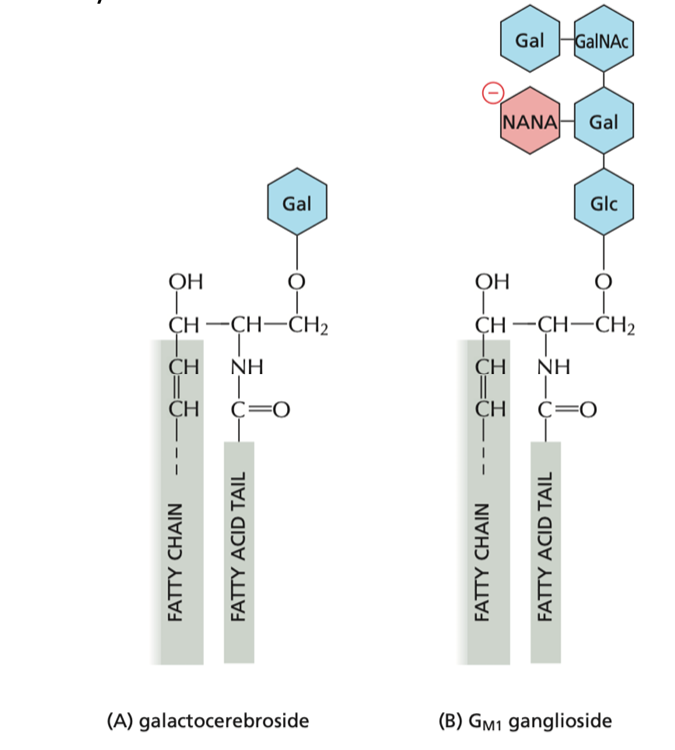
\includegraphics[width=0.3\linewidth]{glycolipids.png}
            \caption{glycolipid structure}
            \label{fig:enter-label}
        \end{figure}
        Glycolipids are lipids that have been modified by adding a sugar. This modifiation can be sequencial meaning that there can be more than one sugar added to form very complex R-groups. \textbf{Glycolipids are on the outside of the cell membrane}

    
        \paragraph{sterols}
        \begin{figure}[H]
            \centering
            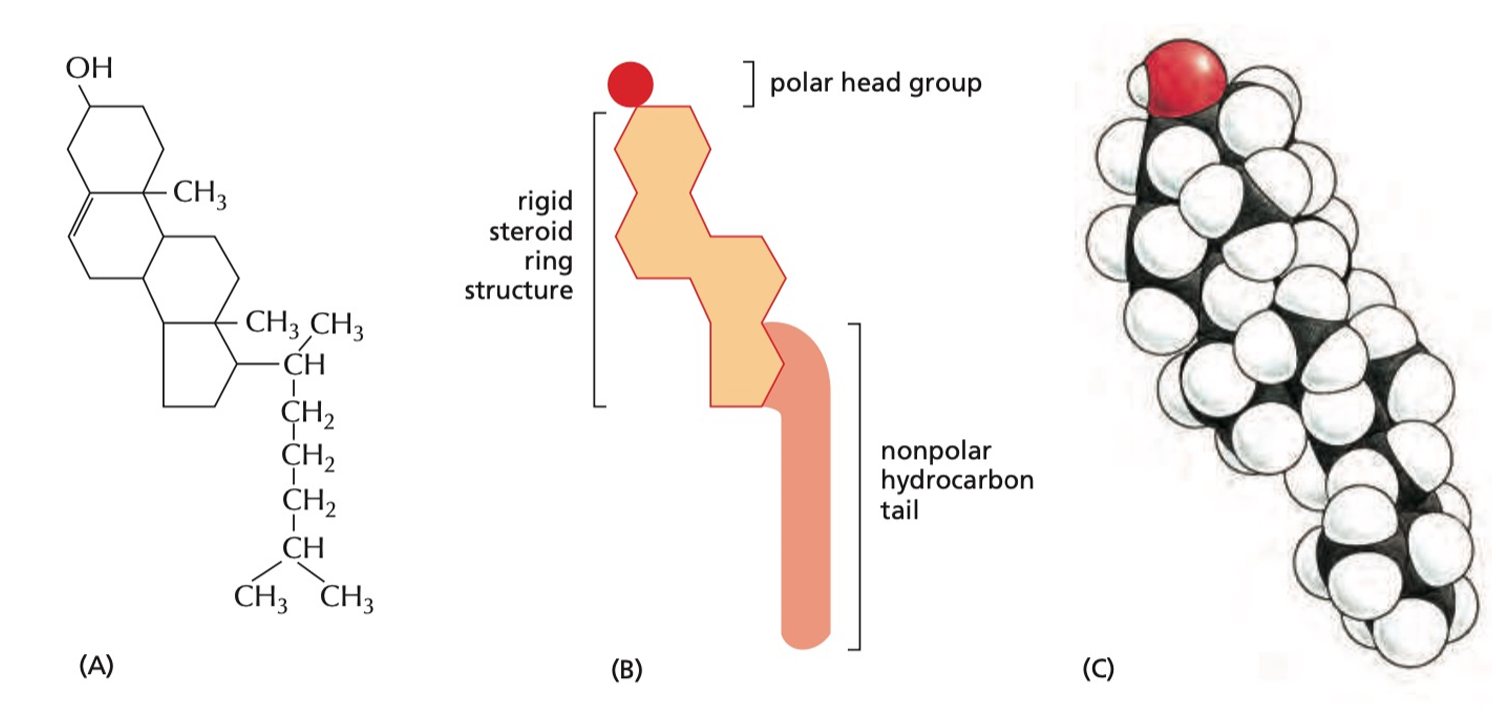
\includegraphics[width=0.5\linewidth]{sterols.png}
            \caption{sterols structure}
            \label{fig:enter-label}
        \end{figure}
        This class of lipids consist of of a \textbf{rigid ring structure and a polar head group}. The posterboy for this group is \textbf{cholesterol}, which incorportates in the membrane to change it's fluidity by incorporating between phospholipids therby stiffening the membrane.
        \begin{figure}[H]
            \centering
            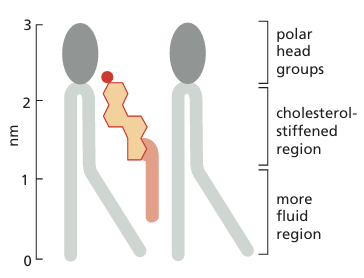
\includegraphics[width=0.3\linewidth]{cholesterolStiffening.png}
            \caption{cholesterol stiffens the membrane by incorporating itself between two phospholipids}
            \label{fig:enter-label}
        \end{figure}

        \subsubsection{lipid composition of common cells}
        \begin{figure}[H]
            \centering
            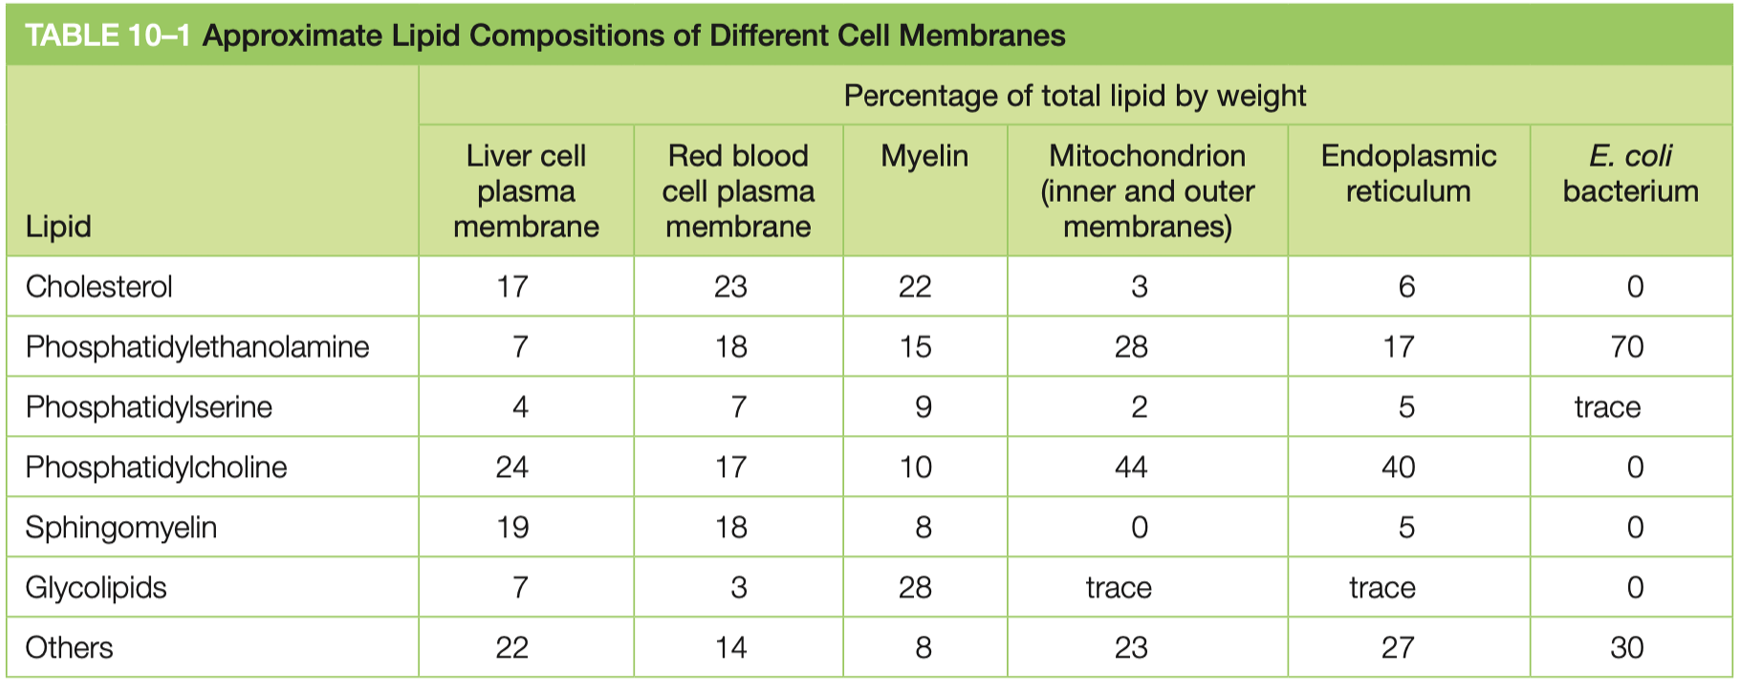
\includegraphics[width=\linewidth]{table.png}
            \caption{table of lipid composition and it's cell type variation}
            \label{fig:lipidComposition}
        \end{figure}
        
        

            

    

    \subsection{Properties of Cell Membranes are dynamic}
        lipids are incredibly diverse set of molecules that are made in an equally complex process. This diversity gives the cell many mechanisms to influence the membranes properties.
        
        \subsubsection{saturated vs unsturated and tail length}
        The \textbf{amount of cis-double bonds} affects membrane stiffness. The higher the amount of cis Double bonds the harder it is to pack the molecules together making the membrane more fluid. 
        \par
        Another way to affect fluidity is by the length of the fatty acid tails. the longer the tail the stronger the Van der waals forces, thus making the membrane less fluid.


        \subsubsection{Temperatures effect on the membrane}
        \begin{figure}[H]
            \centering
            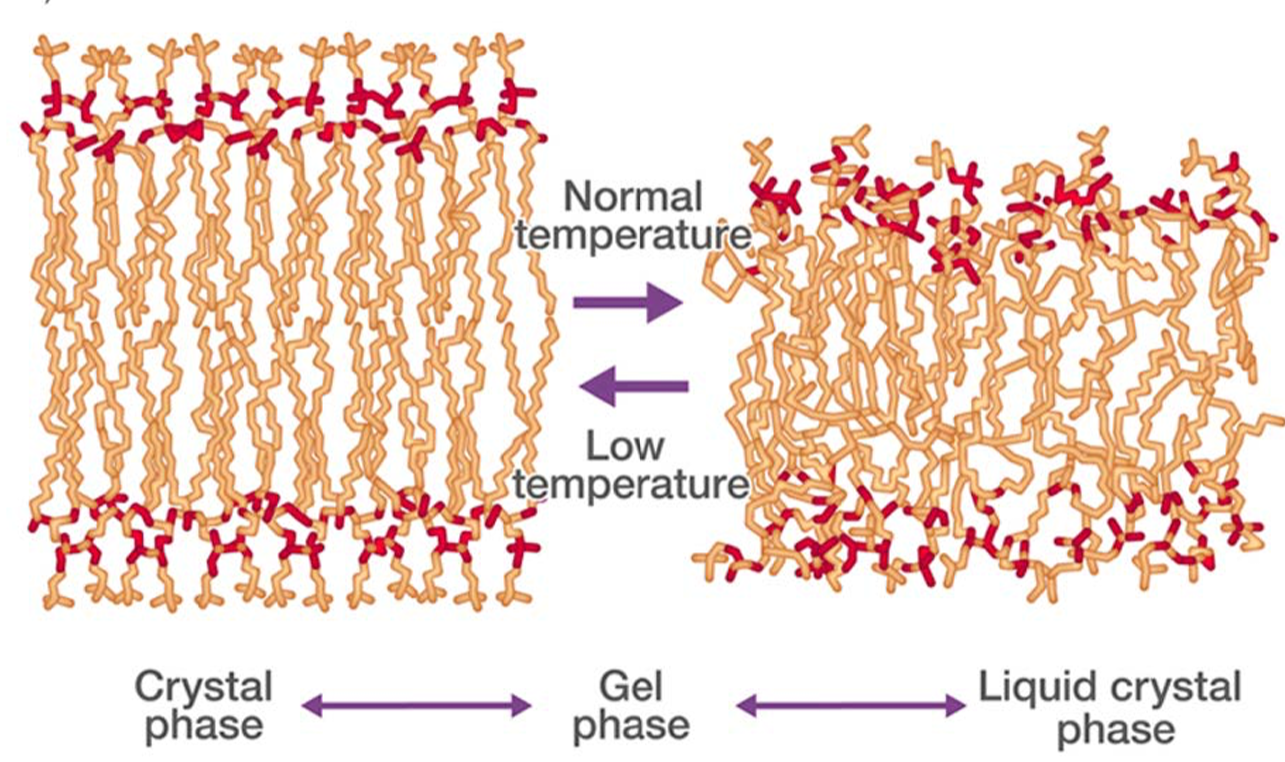
\includegraphics[width=0.4\linewidth]{temp.png}
            \caption{temperature on the membrane rigidity}
            \label{fig:enter-label}
        \end{figure}

        The temperture an organism is exposed to inpacts it's rigidity. Thus the saturation/ length of fatty acids can be used to adapt to the enviroment. \textbf{This means that animals living in cold have different membrane compositions}


    \subsection{Movement of Lipids in Cell Membranes}
        \begin{figure}[H]
            \centering
             % First subfigure (side by side)
            \subfigure[membrane fluidity visualized]{
                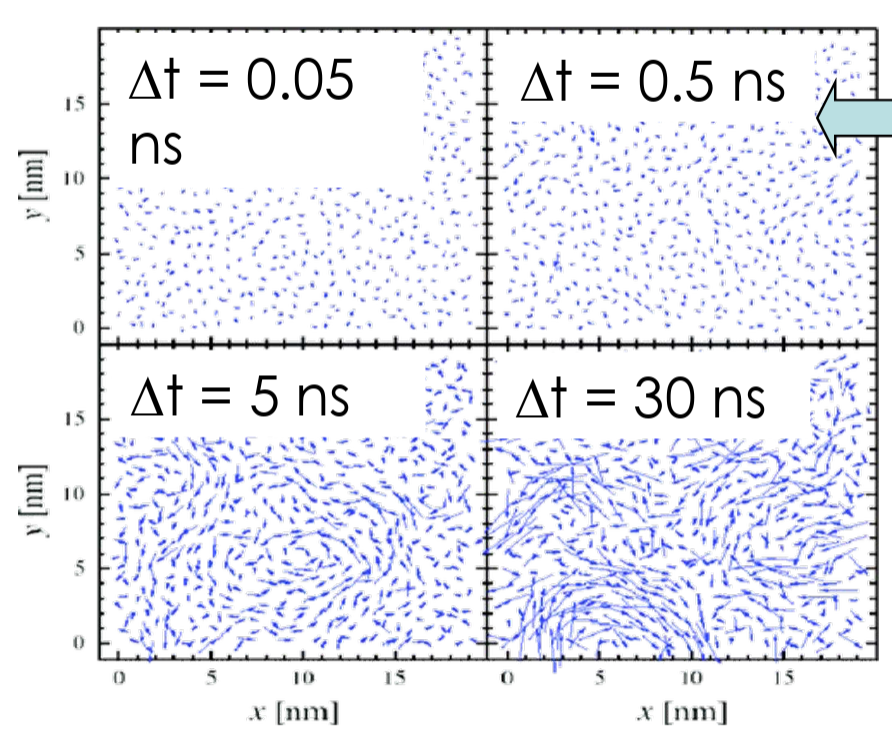
\includegraphics[width=0.35\linewidth]{fluidty.png}
                \label{fig:fluidity}
            }
            \hspace{0.05\textwidth} % Adds a small horizontal space between the figures
            % Second subfigure (side by side)
            \subfigure[asymetrical distribution between the two leaflets]{
                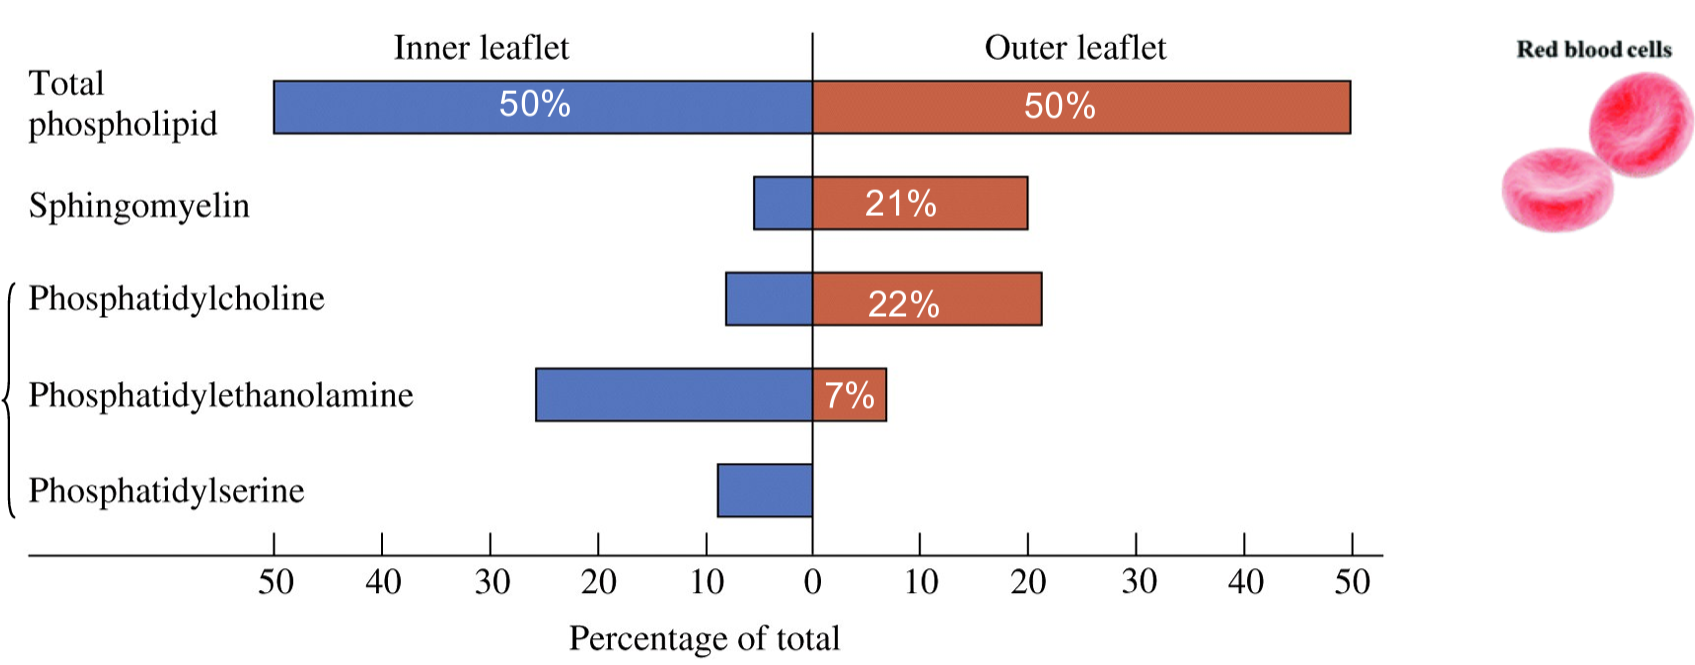
\includegraphics[width=0.55\linewidth]{asymetrical.png}
                \label{fig:asymetrical}
            }
           

            \subfigure[types of movements possible for individual phospholipids]{
                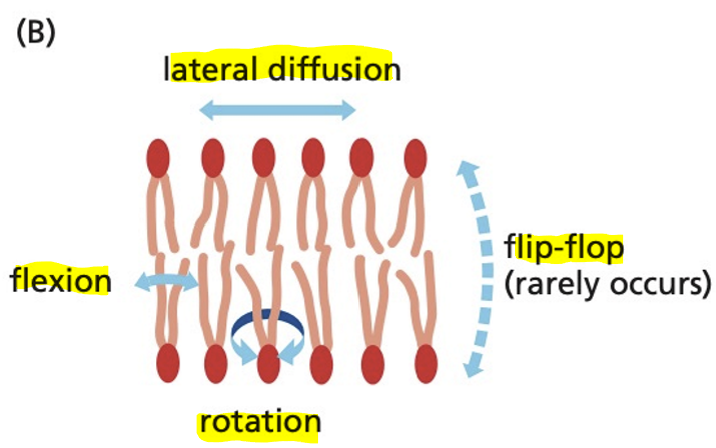
\includegraphics[width=0.3\linewidth]{lipid movement.png}
                \label{fig:asymetrical}
            }

             \caption{membrane fluidity and asymetry}
        \end{figure}
    
        
    Membranes are very mobile. The lipids rapidly diffuse and move around on both of the \textbf{leaflets}. They tend to move together and form wave like patterns much like the ocean (albeit a kinda gross and fatty ocean)
    \par
    The lipids \textbf{rarely flip between the leaflets} This means that there is an \textbf{asymetric distribution of various lipids between the inner and outer leaflet as they are produced at different locations}. The cells has enzymes called\textbf{ flipases that move the cells from one leaflet to another}. The other type of enzyme are called \textbf{scramblases that indiscriminately move lipids around between the leaflets}
       
    \subsection{Lipid Rafts}
    \begin{figure}[H]
        \centering
        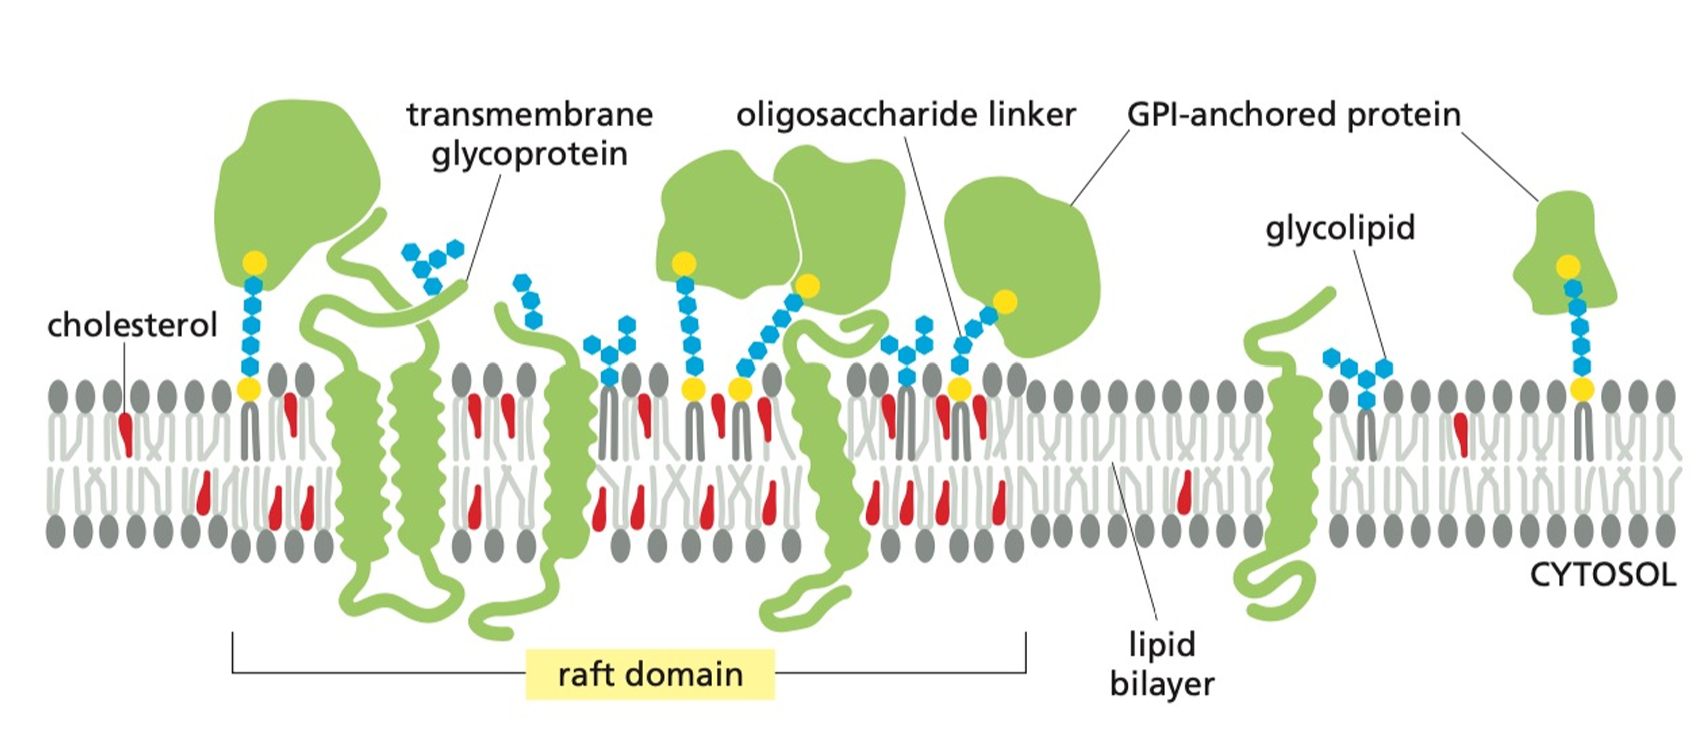
\includegraphics[width=1\linewidth]{rafts.png}
        \caption{raft domains}
        \label{fig:enter-label}
    \end{figure}

    \textbf{\gls{lateralphaseseparation}} is a phenomenon where sphingomyelin and cholesterol seem to group together into larger units called \textbf{Lipid rafts}. This phenomenon apears in vivo but to a much smaller extent than in artificial membranes. These domains have been theorised to play a role in cell localisation, where the difference in thickness will force larger transmembrane helixes to go to these rafts domains.


\end{document}

